\section{Descripción de circuito con diferentes operadores de asignación (modificado) \label{sec:s2}}

\begin{center}
	\begin{minipage}{12cm}
		\begin{tcolorbox}[title=Actividad 2]
			Cambiar el operador de asignación de la segunda sentencia dentro del bloque \textit{"always"}. Compilar y observar el resultado de la síntesis con el visor RTL. Comparar con el resultado del inciso 1.
		\end{tcolorbox}	
	\end{minipage}
\end{center}

La visualización RTL del circuito modificado con múltiples asignaciones, descrito en Verilog, se muestra en la \autoref{fig:a_circuit2_rtl}. La implementación se hace empleando las mismas compuertas lógicas y Latches, no obstante, la conexión es diferente, siendo que, una de las entradas de compuerta XOR proviene de la salida de la compuerta OR de la señal \textit{Select}, y no del Latch dispuesto para la misma señal. Las simulaciones se visualizan en la \autoref{fig:a_circuit2_wave}, en donde se muestra que el módulo opera de manera diferente, en comparación con el módulo anterior.

En los Anexos se localiza la descripción en Verilog de este módulo. En el código solo se realiza la modificación de la señal \textit{Select}, utilizando un operador de asignación bloqueante.

\begin{figure}[ht]
	\centering
	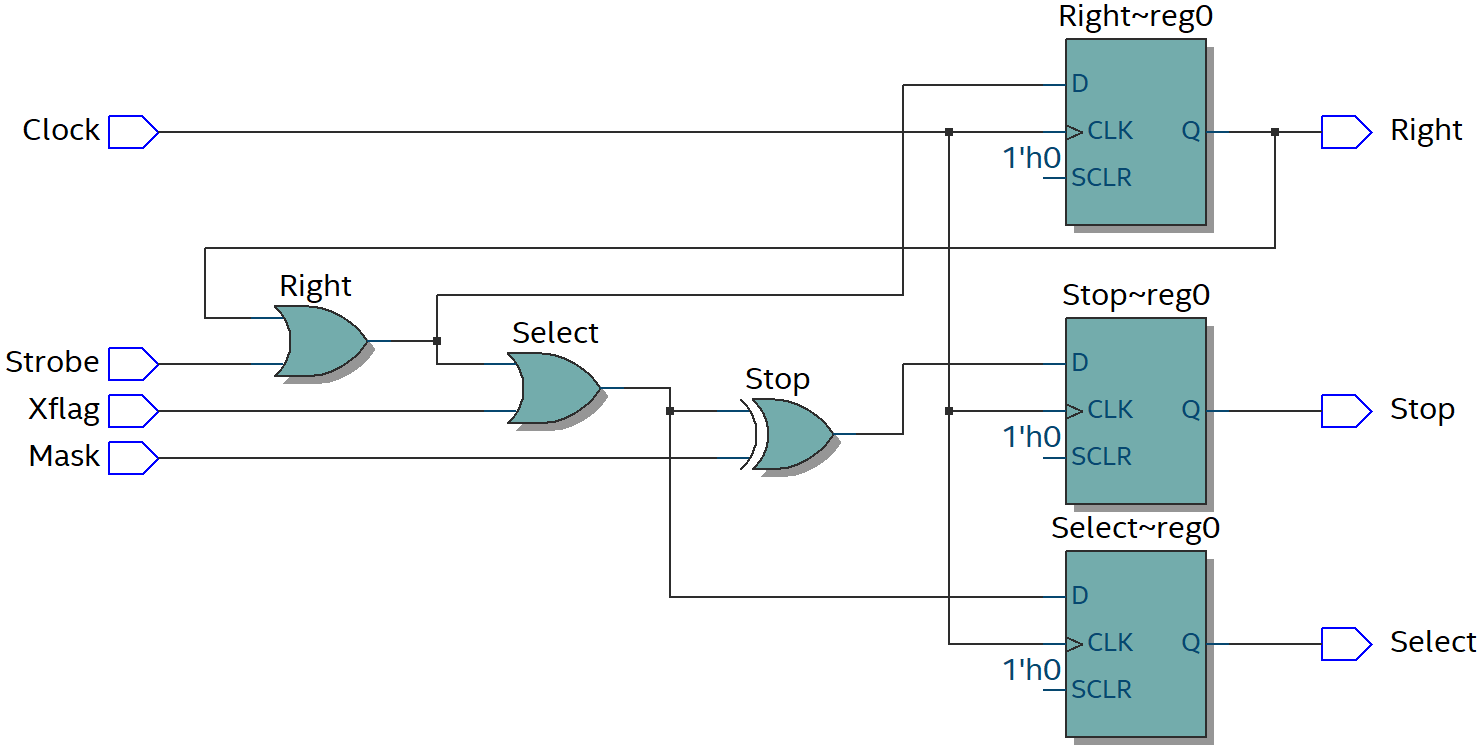
\includegraphics[scale=0.23]{Assignment_Circuit2_RTL.png}
	\caption{Diagrama RTL del circuito con múltiples asignaciones, descrito en Verilog (versión modificada). \label{fig:a_circuit2_rtl}}
\end{figure}

\begin{figure}[ht]
	\centering
	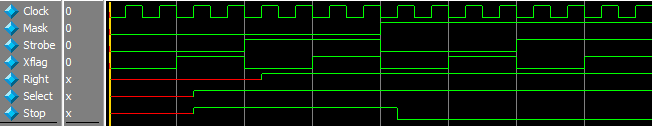
\includegraphics[scale=0.7]{Assignment_Circuit2_Wave.png}
	\caption{Simulación del circuito con múltiples asignaciones, descrito en Verilog, con el visor de formas de onda de ModelSim (versión modificada). \label{fig:a_circuit2_wave}}
\end{figure}